%%%%%%%%%%%%%%%%%%%%%%% file template.tex %%%%%%%%%%%%%%%%%%%%%%%%%
%
% This is a general template file for the LaTeX package SVJour3
% for Springer journals.          Springer Heidelberg 2010/09/16
%
% Copy it to a new file with a new name and use it as the basis
% for your article. Delete % signs as needed.
%
% This template includes a few options for different layouts and
% content for various journals. Please consult a previous issue of
% your journal as needed.
%
%%%%%%%%%%%%%%%%%%%%%%%%%%%%%%%%%%%%%%%%%%%%%%%%%%%%%%%%%%%%%%%%%%%
%
% First comes an example EPS file -- just ignore it and
% proceed on the \documentclass line
% your LaTeX will extract the file if required
\begin{filecontents*}{example.eps}
%!PS-Adobe-3.0 EPSF-3.0
%%BoundingBox: 19 19 221 221
%%CreationDate: Mon Sep 29 1997
%%Creator: programmed by hand (JK)
%%EndComments
gsave
newpath
  20 20 moveto
  20 220 lineto
  220 220 lineto
  220 20 lineto
closepath
2 setlinewidth
gsave
  .4 setgray fill
grestore
stroke
grestore
\end{filecontents*}
%
\RequirePackage{fix-cm}
%
%\documentclass{svjour3}                     % onecolumn (standard format)
%\documentclass[smallcondensed]{svjour3}     % onecolumn (ditto)
\documentclass[smallextended]{svjour3}       % onecolumn (second format)
%\documentclass[twocolumn]{svjour3}          % twocolumn
%
\smartqed  % flush right qed marks, e.g. at end of proof
%
%\usepackage[round, sort, numbers]{natbib}
\usepackage{graphicx}   % omit 'round' option if you prefer square brackets
% \usepackage{mathptmx}      % use Times fonts if available on your TeX system
%
% insert here the call for the packages your document requires

\usepackage{amsmath}
\usepackage{amsfonts}
\usepackage{amssymb}
\usepackage{eurosym}
\usepackage{mathtools}
\usepackage{graphicx}
\usepackage{rotating}
\usepackage{setspace}
\usepackage{color}
\usepackage{fancyhdr}
\usepackage{ragged2e}
\usepackage{appendix}
\usepackage{tabularx}
\usepackage{multirow}
\usepackage{booktabs}
\usepackage{xfrac}
\usepackage{pgfplots}
\usepackage{url}
\usepackage{emptypage}
\usepackage{wrapfig}
\usepackage{dsfont}
\usepackage{soul}
\usepackage[dvipsnames]{xcolor}
\usepackage{csquotes}
\usepackage{hyperref}
\usepackage{xcolor}
\usepackage{todonotes}


%
% please place your own definitions here and don't use \def but
% \newcommand{}{}
%

\newcommand{\gr}[2][]{\todo[color=violet!40!,#1]{\textsf{GR:} #2}}
\newcommand{\bm}[2][]{\todo[color=blue!20,#1]{\textsf{BM:} #2}}


\newtheorem{assumption}{Assumption}
\newtheorem{prop}[theorem]{Proposition}
\newtheorem{observation}[theorem]{Observation}


\DeclareMathOperator{\diag}{diag}
\DeclareMathOperator{\dw}{d_w}
\DeclareMathOperator{\C}{C_{tc}}
\DeclareMathOperator{\T}{T}
\DeclareMathOperator{\MP}{MP}
\DeclareMathOperator{\KP}{KP}
\DeclareMathOperator{\K}{K}
\DeclareMathOperator{\Id}{Id}
\DeclareMathOperator{\SSpan}{Span}
\DeclareMathOperator{\epi}{epi}
\DeclareMathOperator{\supp}{supp}


%\numberwithin{definition}{section}
\numberwithin{theorem}{section}
%\numberwithin{problem}{section}
\newcommand{\nc}{\newcommand}
\nc{\boB}{{\mathbf{B}}}
\nc{\boL}{{\mathbf{L}}}
\nc{\boY}{{\mathbf{Y}}}
\nc{\boI}{{\mathbf{I}}}
\nc{\boV}{{\mathbf{V}}}
\nc{\boS}{{\mathbf{S}}}
\nc{\tV}{{\Tilde{{V}}}}
\nc{\tI}{{\Tilde{{I}}}}
\nc{\tY}{{\Tilde{{Y}}}}
\nc{\tS}{{\Tilde{{S}}}}
\nc{\fr}{{\rightarrow}}
\nc{\co}{{\nabla}}
\nc{\E}{\mathbb{E}}
\nc{\CG}{C_{\Sigma}^{\text{Gauss}}}
\nc{\var}{Var}
\nc{\rows}{S}
\nc{\cols}{R}
\nc{\rowP}{\sigma}
\nc{\colP}{\delta}
\nc{\rowW}{\omega}
\nc{\colW}{\tau}

\nc{\sS}{ \mathscr{S}}
\nc{\sC}{ \mathscr{C}}
\nc{\cH}{{\mathcal H}}
\nc{\cR}{{\mathcal R}}
\nc{\cA}{{\mathcal A}}
\nc{\cG}{{\mathcal G}}
\nc{\cC}{{\mathcal C}}
\nc{\cD}{{\mathcal D}}
\nc{\cO}{{\mathcal O}}
\nc{\cI}{{\mathcal I}}
\nc{\cB}{{\mathcal B}}
\nc{\cY}{{\mathcal Y}}
\nc{\cK}{{\mathcal K}} 
\nc{\cX}{{\mathcal X}}
\nc{\cS}{{\mathcal S}}
\nc{\cE}{{\mathcal E}}
\nc{\cF}{{\mathcal F}}
\nc{\cZ}{{\mathcal Z}}
\nc{\cQ}{{\mathcal Q}}
\nc{\cP}{{\mathcal P}}
\nc{\cL}{{\mathcal L}}
\nc{\cM}{{\mathcal M}}
\nc{\cN}{{\mathcal N}}
\nc{\cT}{{\mathcal T}}
\nc{\cW}{{\mathcal W}}
\nc{\cU}{{\mathcal U}}
\nc{\cJ}{{\mathcal J}}
\nc{\cV}{{\mathcal V}}
\nc{\bH}{{\mathbb H}}
\nc{\bA}{{\mathbb A}}
\nc{\bG}{{\mathbb G}}
\nc{\bC}{{\mathbb C}}
\nc{\bO}{{\mathbb O}}
\nc{\bI}{{\mathbb I}}
\nc{\bB}{{\mathbb B}}
\nc{\bY}{{\mathbb Y}}
\nc{\bK}{{\mathbb K}} 
\nc{\bX}{{\mathbb X}}
\nc{\bS}{{\mathbb S}}
\nc{\bE}{{\mathbb E}}
\nc{\bF}{{\mathbb F}}
\nc{\bZ}{{\mathbb Z}}
\nc{\bQ}{{\mathbb Q}}
\nc{\bN}{{\mathbb N}}
\nc{\bP}{{\mathbb P}}
\nc{\bL}{{\mathbb L}}
\nc{\bM}{{\mathbb M}}
\nc{\bT}{{\mathbb T}}
\nc{\bW}{{\mathbb W}}
\nc{\bU}{{\mathbb U}}
\nc{\bD}{{\mathbb D}}
\nc{\bJ}{{\mathbb J}}
\nc{\bV}{{\mathbb V}}
\nc{\bR}{{\mathbb R}}


\newcommand{\virgolette}[1]{``#1''} %\virgolette{questo č fra virgolette}%
%\usepackage{frontespizio}
\newcommand{\abs}[1]{\lvert#1\rvert}



% Insert the name of "your journal" with
\journalname{Optimization and Engineering}
%
\begin{document}


\title{Modelling of a fully renewable energy grid with hydrogen storage: time aggregation for a scalable Capacity Expansion Problem
%\thanks{Grants or other notes
%about the article that should go on the front page should be
%placed here. General acknowledgments should be placed at the end of the article.}
}
%\subtitle{}%A stochastic approach considering time interdependence of wind and solar power.}

\titlerunning{Time aggregation for a scalable CEP}        % if too long for running head

\author{Bianca Urso \and Gabor Riccardi}

%\authorrunning{Short form of author list} % if too long for running head

\institute{B. Urso \at
              IUSS School of Advances Studies, Palazzo del Broletto, Piazza della Vittoria, 15 – 27100 Pavia PV, Italy\\
              Tel: +39 0382 375811\\
              Fax: +39 0382 375899\\
              \email{bianca.urso@iusspavia.it}           %  \\
%             \emph{Present address:} of F. Author  %  if needed
           \and
           G. Riccardi \at
           Dipartimento di Matematica ”F. Casorati”
           Via Adolfo Ferrata, 5 – 27100 Pavia
}

\date{Received: date / Accepted: date}
% The correct dates will be entered by the editor


\maketitle


\begin{abstract}
  In recent years, the integration of renewable energy sources into electrical grids has become a critical area of research due to the increasing need for sustainable and resilient energy systems. 
  To address the variability of wind and solar power output over time, electricity grids expansion plans need to account for multiple scenarios over large time horizons.
  This significantly increases the size of the resulting Linear Programming (LP) problem, making it computationally challenging for large scale grids. 
  To tackle this, we propose an approach that aggregates time steps to reduce the problem size, followed by an iterative refinement of the aggregation, in order to converge to the optimal solution.
  Using the previous iteration's solution as a warm start, we introduce and compare methods to select which time intervals to refine at each iteration.
  The first method employs a validation function, which evaluates with a Rolling Horizon method the feasibility of the aggregated solutions and selects the time interval on which the validation fails. 
  The second method uses the proportion of net power production in each time step relative to the aggregated time interval. 
  These selection methods are then compared against a random interval selection approach. 

  \keywords{Electric power system \and Stochastic Programming \and Rolling Horizon \and Time aggregation \and Renewable Energy}
  \subclass{90-10 \and 90B15 }

\end{abstract}



\newpage
\section{INTRODUCTION}


The threat of climate change is pushing policy-makers to pursue greater integration of renewable energy sources into
 electrical grids, while at the same time ensuring reliability and resilience through digital optimization of electric 
 power distribution and transmission in smart grids \textcolor{green}{\cite{EU_context}}. 
One of the main difficulties arising when designing an electric power system relying on renewables is the great variability
 of the generation of electricity through wind and solar, since these resources are highly dependent on weather conditions. 
To deal with this variability, a possible solution gaining a lot of traction in recent years is the introduction of an energy
 storage system relying on hydrogen, converting energy from hydrogen to electricity and vice versa in fuel cells and 
 elecrolyzers \textcolor{green}{\cite{INTRO_blanco}, \cite{INTRO_parra}}. 
It is of interest to evaluate the optimal solution, in terms of investment plan, to supply the grid along with industrial
 hydrogen demand in a dependable way. 
The stochastic nature of the problem though makes it impossible to plan long-term by optimizing on forecasts, and requires
 a statistical approach to ensure a robust model.

Up to now, common approaches have adopted Stochastic Programming (SP) or Robust Optimization (RO) models, along with hybrid
 models involving Information Gap Decision Theory or Chance Constraint \textcolor{green}{\cite{review_math_opt}}. 
While initially favored, the SP approach comes with high computational burden, so RO models have seen more popularity 
in recent years, despite the drawback of being conservative methods with higher average cost of operation and planning of energy systems.

In the typical setting, the problem to solve is a Capacity Expansion Problem (CEP) regarding infrastructure investments:
 solar and wind farms, fuel cells, hydrolizers, grid upgrades to augment Net Transfer Capacity (NTC) and so on. 
Nested within the CEP is an Economic Dispatch (ED) problem concerning the operational costs of said infrastructure. 
The problem is well suited to be modelled through mixed integer linear programming (MILP), as is explained in detail in 
\textcolor{green}{\cite{INTRO_isolated_MIP}} and \textcolor{green}{[?]}.%\textcolor{green}{\cite{Dagdougui}}. 

The CEP for investment planning requires to look at long time horizons, and on the other hand intra-day variability in generation is the main complexity driver for the ED problem, so the time horizon must be modelled by a large quantity of fairly tight time steps. 
Furthermore, Large scale grids can be modelled with various degrees of spacial aggregation, as is explored in \textcolor{green}{\cite{Horsch}} and \textcolor{green}{\cite{BIENER2020106349}}, and problem size increases more than linearly with the number of nodes.
Thus the temporal and spacial characteristics of the model bring the MILP size to increase rapidly. 
This is especially demanding in the case of SP, since all the variables from the inner ED problem must be reproduced over all scenarios.

To reduce these costs, one possible approach is to use a Rolling Horizon (RH). 
The basic technique is described in \textcolor{green}{\cite{INTRO_Glomb}}, along with some results regarding quality guarantees for the optimality of the solution. 
In \textcolor{green}{\cite{INTRO_Palma-Behnke}}, a rolling horizon approach is used within a RO model to optimize the operation of a micro-grid composed of two PV systems, a wind turbine, a diesel generator and a lead-acid battery for storage, serving an isolated area in Chile. 
A similar idea is applied in \textcolor{green}{\cite{INTRO_karlsruhe}}, 
where integer variables representing capital investments are initially relaxed 
and then progressively fixed in successive time steps, reducing the computational
 costs associated to the search for integer solutions.

A big drawback of the RH approach is that the solution it provides is not optimal on the whole time horizon. 
Indeed \textcolor{green}{\cite{INTRO_short-term}} explores the effect of short-term planning with limited foresight
 compared to perfect foresight optimizaion. 
On the other hand, the RH approach better reflects actual decision making based on information that is only available
 progressively, which is the case for the management of energy system planning relying on weather forecasts.

In our work, we build a LP model of a large scale electrical grid powered by wind and solar power generation and supported
 by hydrogen storage. 
The LP aims to solve the CEP for the design of the grid, stochastically on the scenarios for the inner ED problem. 
A RH method is then proposed for the validation of the results for the CEP obtained in the perfect foresight optimization, rather than as a 
stand-alone technique, to ensure that given a solution to the CEP, the ED problem admits feasible solutions even in a limited-foresight environment. 
The idea is to solve the CEP as to build a grid that can be operated as a ``smart grid'', through a control system that
 optimizes on day ahead forecasts.

 Further, we present our attempt at dealing with the great computational requirement by aggregating on time steps to reduce the model size. 
 The optimization is carried out through an iterative procedure gradually refining the partition of the time horizon, and converging to the optimal solution.
To guide the selection of these progressively tighter relaxations of the perfect foresight model, two methods are discussed and compared:
a first one making use of the aforementioned RH validation function, and a second one devised ad hoc based on the problem structure.


%\color{gray}
%Finally, to generate the scenarios needed to train and test the SP model, a Gaussian Copula method was used. 
%This has been previously done by \textcolor{violet}{\cite{INTRO_GaussCopula}}.


This paper is organized as follows. 

Section \ref{section: model} descibes the formulation of the LP problem: the first subsection details the perfect foresight model, and the second adapts the structure from the first to the RH approach. 

Section \ref{section:time-resolution} deals with time aggregation. In subsection \ref{subsection: relax} the LP problem associate to the variables aggregated over time is defined, and is shown to be a relaxation of the disaggregated one; 
In subsection \ref{subsection: iter} a method is proposed to iterate through progressively finer time aggregations, in order toconverge to the optimal perfect foresight solution. The use of the RH method defined in the previous section is proposed to select the interval to disaggregate. 
In subsection \ref{subsection: rho}, the structure of the constraint matrix is exploited to derive conditions under which the aggregated solution is feasible for the disaggregated problem, and the result is used to devise a heuristic for the disaggregation selection. 

\textcolor{red}{
  Section \ref{section: comp res} contains the computational results: some example outputs from the perfect foresight LP are explored, then the three aggregation-iteration methods are compared over time and number of iterations for convergence.
}
%\textcolor{gray}{An appendix is given detailing the scenario generation method used to generate the input scenarios for the model. }




%=================================================================================================================================================================================================================================================================================================================
%=================================================================================================================================================================================================================================================================================================================

%=================================================================================================================================================================================================================================================================================================================
%=================================================================================================================================================================================================================================================================================================================






\section{MODEL}\label{section: model}

\subsection{LP Formulation}\label{subsection: LP}
Our model describes a network in Europe that is to be powered and supplied of hydrogen trough power generated by photovoltaic panels and wind turbines, converted to hydrogen through electrolysis and potentially reconverted in fuel cells.

The network is represented by an undirected multigraph \(\cG = (\cN, \cE)\), where \(\cN\) corresponds to the nodes in the network, and \(\cE = \cE_H \cup \cE_P\) represents transmission lines (\(e \in \cE_P\)) and hydrogen lines (\(e \in \cE_H\)).
Each of these nodes can be in different countries in Europe, and the power generated by wind and solar power depends on the node location. 
In particular, if node \(n \in \cN\) is in France, the scenarios for power generation at \(n\) will be generated using parameters fitted to France's data.

Each node has its generators, hydrogen storage, fuel cells and hydrolyzers, for which the capacity is to be decided. 
Likewise, the CEP aims to solve for transmission line NTC and hydrogen pipe transmission capacity for each edge of the network. 
The basic formulation of the LP described in this subsection allows us to solve the CEP with perfect foresight. 

We decided to model our problem as a LP problem instead of MILP, as would be standard in the literature. 
This is because when modelling a large grid with high demand, optimizing on continuous variables and then rounding up to the closest integer for variables regarding the number of PV panels and turbines notably decreases computational costs, without relevant difference in the final cost. 
The same wouldn't be possible when optimizing over micro-grids.

The model takes in input the generation and load scenarios of the given area along with various parameters indicating costs and efficiency of the current state of technology and possible upper bounds for the decision variables. 
The CEP and the ED problems for all scenarios are solved concurrently. 
When optimizing over multiple scenarios jointly, the solver returns the minimal amount of infrastructure and capacities that is needed to have feasibility (that is, demand met at all time and no blackouts) over all scenarios in input, with minimal cost. 
Cost is considered to be the sum of capital costs and average operational costs of the infrastructure over the scenarios.

For the rest of this article, when talking about a solution to the LP problem, we refer to a realization of variables solving the CEP and ED problem jointly. 
When mentioning a solution to the CEP problem, we refer to those components of the corresponding LP problem solution that are not time or scenario dependent. 
When talking about a solution to the ED problem only, we refer to a realization of the time and scenario dependent variables that solve the problem for a given \textit{fixed} CEP solution.

The optimization problem is solved using the Gurobi solver \textcolor{green}{\cite{INTRO_gurobi}}.


%%%%%%%%%%%%%%%%%%%%%%%%%%%%%%%  VARIABLES  %%%%%%%%%%%%%%%%%%%%%%%%%%%%%%%%%%%%%

\subsubsection{Decision Variables}

The main variables that are of interest to the policy maker are, for each location $n$, the number of wind turbines and PV panels to install, as well as hydrogen storage capacity.
Stored hydrogen is considered to be the total of liquid and gas hydrogen to be stored. 
Our model does not assume a distinction between the two forms, and considers hydrogen to be immediately ready for long-term storage as soon as it is converted from electricity, as well as instantaneously convertible to electricity in fuel cells at need. 
For more detailed models of the management of hydrogen see \textcolor{green}{[?]}.

Important values to consider when planning the grid are the power capacity and conversion speed of fuel cells and electrolyzers: variables $mhte_n$ and $meth_n$, indexed by node $n$, indicate for each location the maximum amount of energy that can be converted at a single time step respectively from hydrogen to electricity and vice versa. 
These values are essential to estimate in order to design a grid that can effectively accommodate peak production and supply during low production periods.

Transmission on the grid lines is considered to be bound by Net Transfer Capacity (NTC) \textcolor{green}{[?]}. 
Existing NTC is estimated through the procedure followed by \textcolor{green}{\cite{tesi_NTC}}, by collecting data from \textcolor{green}{\cite{entsoe_NTC}}. 
Improvements on the existing capacity for power lines or hydrogen transport infrastructure are considered through variables $addNTC_l$ and $addMH_l$.
Indeed, upgrades to the European grid's transfer capacity are currently considered a key element for the integration of renewables \textcolor{green}{[?]}.

Variables linked to the inner ED problem are indexed by scenario \(j\in J\), time step \(t\in\{1...T\}\), and either node \(n \in \cN\) or edge $l\in\cE_H$ or $l \in \cE_P$. 
For the variables pertaining to transmission on an edge, two distinct variables are considered, one for each direction. 
This way, all variables are set to be non-negative. This will be relevant for the formulation of the time-aggregated relaxation of the LP problem.

See Table \ref{table_vars} for the summary of all decision variables.

\begin{table}
  \caption{Decision variables}
  \label{table_vars}
  \begin{tabularx}{\textwidth}{ccl}
  \hline\noalign{\smallskip}
  \textbf{Name} & \textbf{Unit} & \textbf{Description}  \\
  \noalign{\smallskip}\hline\noalign{\smallskip}
  $\text{ns}_n$ & - & Number of solar units at node $n \in \cN$ \\
  $\text{nw}_n$ & - & Number of wind units at node $n \in \cN$ \\
  $\text{nh}_n$ & kg & Storage capacity at node $n \in \cN$\\
  $\text{mhte}_n$ & kg & \parbox[t]{0.70\textwidth}{Maximum hydrogen to electricity capacity,  at node $n \in \cN$} \\
  $\text{meth}_n$ & MWh & Maximum electricity to hydrogen capacity at node $n \in \cN$\\
  $\text{addNTC}_l$ & MWh & Additional net transfer capacity on line $l\in\cE_P$\\
  $\text{addMH}_l$ & kg & Additional hydrogen transfer capacity on pipe $l\in\cE_H$\\
  \noalign{\smallskip}\hline\noalign{\smallskip}
  $\text{H}_{j,t,n}$ & kg& Stored hydrogen at node $n$, time \(t\), scenario \(j\)\\
  $\text{HtE}_{j,t,n}$ & kg& Hydrogen converted to electricity at time \(t\),scenario \(j\) \\
  $\text{EtH}_{j,t,n}$ & MWh& Electricity converted to hydrogen at time \(t\), scenario \(j\)\\
  P\_edge$^+_{j,t,l}$&MWh& Power passing through line $l$ at time $t$, scenario $j$ \\
  P\_edge$^-_{j,t,l}$&MWh& Power passing through line $l$ at time $t$, scenario $j$ \\
  H\_edge$^+_{j,t,l}$&kg& Hydrogen transported through line $l$ at time $t$, scenario $j$\\
  H\_edge$^-_{j,t,l}$&kg& Hydrogen transported through line $l$ at time $t$, scenario $j$\\
  \noalign{\smallskip}\hline
  \end{tabularx}
  \end{table}
  
%%%%%%%%%%%%%%%%%%%%%%%%%%%%%%%  PARAMETERS  %%%%%%%%%%%%%%%%%%%%%%%%%%%%%%%%%%%%%


\subsubsection{Parameters}

There are numerous parameters that describe the grid and are passed to the model. 
The main ones are related to capital costs of the infrastructure to be built and the following values are assumed for panels and turbines: $cs = 400$\euro, $cw = 3 000 000$\euro. 
We also set capital costs for fuel cells and electrolyzers: since hydrogen infrastructure is usually obtained by reconverting existing infrastructure from other purposes, the estimation of investment costs is very location dependent and beyond the scope of this work \textcolor{green}{[?]}. 
Thus for our purposes, instead of representing the actual investment for the facilities, a minimal ``symbolic'' cost is assigned per unit of capacity, so that in minimizing the model estimates needed conversion capacities $mhte_n$ and $meth_n$.

The storage of the hydrogen has a cost that depends on various factors: capital cost of the technology used for storage, operating costs, length of time that the hydrogen is kept in storage.
For our model we only set the parameters $ch$, to be multiplied by the maximum storage needed ($nh$), representing capital cost of storage infrastructure. 
We ignore marginal costs of keeping the hydrogen stored.

In this model we assume no marginal costs for PV and wind power production: the operating costs of the farms throughout their life-cycle can be factored into the capital costs, and there is no additional cost linked to the production itself.

Conversely, the marginal costs of conversion within electrolyzers and power cells are relevant. 
According to the European Hydrogen Market Landcape November 2023 Report \textcolor{green}{\cite{European_H2_Market_landscape}}, ``Hydrogen production costs via electrolysis with a direct connection to a renewable energy source in Europe vary from 4.18 to 9.60 €/kg H2 of hydrogen, with the average for all countries being 6.86 €/kg H2''. 
For electrolyzers, we consider the Levelised cost of hydrogen (LCOH)  to account for both marginal costs and capital costs. 
Such cost is dependent on the country's specific market condition and can be calculated through the European Hydrogen Observator tool \textcolor{green}{\href{https://observatory.clean-hydrogen.europa.eu/tools-reports/levelised-cost-hydrogen-calculator}{[?]}}.

Parameters $fhte_n$ and $feth_n$ are set as scalars between $0$ and $1$ to indicate efficiency of the conversion from hydrogen to electricity and vice versa. 
It is assumed that 1kg of hydrogen has an energy value of 33kWh \textcolor{green}{[?]}. 
Thus if we consider an electrolyzer operating at maximum efficiency ($feth=1$), one MWh of electricity yields 1000/33$\simeq$30kg of hydrogen. 
For our purposes, a standard value of $feth=0.66$ is considered, thus 1MWh yields 20kg of hydrogen. 
Conversely, in a fuel cell operating at maximum efficiency ($fhte=1$) 1kg of hydrogen yields 33kWh. 
We consider a value of $fhte=0.75$, yielding 24.75kWh per kg of hydrogen. Actual efficiencies vary a lot depending on the technology used. 
Furthermore, chemical and physical constraints make it so that efficiencies higher than 0.80-0.85 are currently considered unachievable \cite{DAWOOD}.

Additionally, we assume the flow of electricity has no marginal cost nor power loss (the modelling of that problem is beyond the scope of this project), whereas we do set a cost for the use of hydrogen pipes (or other means of transfer). 
The existing capacity of transmission lines and hydrogen pipes is also set.

Finally, the model allows for upper bounds to be placed on the variables, based on either technological and physical constraints (dimension of the facilities) or because of political choices (e.g. local population unfavourable to wind turbines).

The parameters $ES, EW, EL, HL$, indexed by scenario, time step and node represent the time series of power generation and load values for different scenarios in every node of the grid. 
The method used for generation is described in Appendix \ref{generation}.

See Table \ref{table_param} for the summary of all parameters. 

\begin{table}
\caption{Model parameters}
  \label{table_param}
\begin{tabularx}{\textwidth}{ccl}
  \hline\noalign{\smallskip}
    \textbf{Name} & \textbf{Unit} & \textbf{Description}\\
  \noalign{\smallskip}\hline\noalign{\smallskip}
    cs & \euro& Cost of one Solar Panel at node $n$\\
    cw & \euro & Cost of one Wind Turbine at node $n$\\
    chte$_n$ & \euro/kg & Conversion cost of hydrogen to electricity \\
    ceth$_n$ & \euro/MWh & Conversion cost of electricity to hydrogen \\
    ch$_n$ & \euro/kg & Cost of hydrogen storage capacity\\
    cH\_edge$_l$ & \euro & Cost of transferring 1kg of hydrogen through edge $l\in\cE_H$\\
    cNTC$_l$ & \euro/MWh & Cost of adding NTC to line $l\in\cE_P$\\
    cMH$_l$ &\euro/kg& Cost of adding hydrogen transfer capacity to line $l\in\cE_H$\\
    cmhte & \euro/kg & Cost of needed $HtE$ capacity per unit\\
    cmeth & \euro/MWh&Cost of needed $EtH$ capacity per unit\\
  \noalign{\smallskip}\hline\noalign{\smallskip}
    fhte$_n$ & - & Efficiency of hydrogen to electricity conversion \\ 
    feth$_n$ & - & Efficiency of electricity to hydrogen conversion \\
    NTC$_l$ & MWh & Net Transfer Capacity on line $l\in\cE_P$\\
    MH$_l$ & kg &  Hydrogen transfer capacity on edge $l\in\cE_H$\\
  \noalign{\smallskip}\hline\noalign{\smallskip}
    Mns$_n$ & - & Maximum number of solar panels installable at node $n$\\ 
    Mnw$_n$ & - & Maximum number of wind turbines that can be installed \\ 
    Mnh$_n$ & kg & Maximum hydrogen storage capacity \\
    Mhte$_n$ & kg & Upper bound for \(mhte\) \\ 
    Meth$_n$ & MWh & Upper bound for \(meth\) \\
  \noalign{\smallskip}\hline\noalign{\smallskip}
    ES$_{j,t,n}$ & MWh & Power output of a single solar panel\\
    EW$_{j,t,n}$ & MWh & Power output of a single wind turbine \\
    EL$_{j,t,n}$ & MWh & Electricity load \\
    HL$_{j,t,n}$ & kg & Hydrogen load\\
    \noalign{\smallskip}\hline
\end{tabularx}
\end{table}



%%%%%%%%%%%%%%%%%%%%%%%%%%  OBJECTIVE FUNCTION  %%%%%%%%%%%%%%%%%%%%%%%%%%%%%

\subsubsection{Objective Function}

The cost function is given by the sum of all capital costs of installing infrastructure, plus all marginal costs of the hydrogen to electricity and electricity to hydrogen conversions and hydrogen transfer on the edges at each time step.

Let $d$ be the number of scenarios, and $T$ the number of time steps. The objective function is as follows:
\begin{align*}
    \min \quad 
    &&\sum_{k\in\cN}&(\text{cs}_k \cdot \text{ns}_k+\hspace{-1em}&&\text{cw}_k \cdot \text{nw}_k + \text{ch}_k \cdot \text{nh}_k )\ + \\
    &+& \sum_{k\in\cN}&(\text{cmhte}_k\cdot\text{m} \hspace{-1em}&& \text{hte}_k + \text{cmeth}_k\cdot \text{meth}_k) \ + \\
    &+& \sum_{l\in\cE_P}& (\text{cNTC}_l\cdot \text{ad}\hspace{-1em}&&\text{dNTC}_l) 
    + \sum_{l\in\cE_H} (\text{cMH}_l\cdot \text{addMH}_l) \ + \stepcounter{equation}\tag{\theequation}\label{objVal} \\   
    &+&\frac{1}{d}\sum_{j=1}^{d}&\sum_{t=1}^{T} \Bigg(\sum_{k\in\cN} \hspace{-5em}&&
    (\text{ch\_t}_k \cdot \text{H}_{j,t,k} + \text{chte}_k \cdot \text{HtE}_{j,t,k} + \text{ceth}_k \cdot \text{EtH}_{j,t,k})\ + \\
    &&&\hspace{-2em}&&+\sum_{l\in\cE_H} (\text{cH\_edge}_l\cdot\text{H\_edge}_{j,t,l}) \Bigg)
\end{align*}

The $1/d$ factor in front of the marginal costs allows to average over the scenarios, whereas the capital costs are the same for all scenarios. 
Thus, ignoring the costs of $mhte_k$ and $meth_k$, the objective function value gives an estimate of the actual costs (in \euro) for the set up and maintenance of the system throughout the length of the time horizon. 


%%%%%%%%%%%%%%%%%%%%%%%%%%%%%%%  CONSTRAINTS  %%%%%%%%%%%%%%%%%%%%%%%%%%%%%%%%%%%%%

\subsubsection{Constraints}
The following constraints are to ensure that for all time steps $t$ and all scenarios $j$, the electricity load and the hydrogen load are met. 
The measure units are MWh and kg respectively, and conversion factors are considered for $HtE$ and $EtH$ respecively.
Let $Out(n)$ and $In(n)$ indicate the outgoing and incoming edges from node $n$ on the respective graph. 
For simplicity, we indicate with $P\_edge_{j,t,l}$ the difference of the corresponding variables $P\_edge^+_{j,t,l}-P\_edge^-_{j,t,l}$, and analogously for $H\_edge$. 
When solving, it is sufficient to assign a symbolic cost to them to ensure that only one of them is non zero at each time step. 
Then for each node $n$, scenario $j$ and time step $t$, the following flow balance constraints are imposed:
\begin{align*}
    \text{Electricity Balance:} \quad & \text{ns}_n \cdot \text{ES}\hspace{-1.2em}&_{j,t,n}&+ \text{nw}_k \cdot \text{EW}_{j,t,n} - \text{EL}_{j,t,n} \ + \\
    &  + 0.033\hspace{-2em}& \cdot f&hte_k \cdot \text{HtE}_{j,t,n} - \text{EtH}_{j,t,n}\ + \stepcounter{equation}\tag{\theequation}\label{constr_P}\\
    & + \sum_{l\in Out(n)}\hspace{-1.9em}&\text{P\_}&\text{edge}_{j,t,l} + \sum_{l\in In(n)} \text{P\_edge}_{j,t,l} \ge 0;\\
    \text{Hydrogen Storage:} \quad & \text{H}_{j,t+1,n} \hspace{-5em}&=& \text{H}_{j,t,n} - \text{HL}_{j,t,n}\ +\\ 
    &&& + 30 \cdot feth_k \cdot \text{EtH}_{j,t,n} - \text{HtE}_{j,t,n} \ + \stepcounter{equation}\tag{\theequation}\label{constr_H}\\
    &&& - \sum_{l\in Out(n)}\text{H\_edge}_{j,t,l} + \sum_{l\in In(n)}\text{H\_edge}_{j,t,l}
\end{align*}

We ask that the consumed electricity be less or equal than the produced or received electricity at all times. 
On the grid itself, the two sides should be equal, but we observe that $ns\cdot ES_{j,t} + nw\cdot EW_{j,t}$ indicate the maximum power that can be generated with set weather conditions, whereas actual production will be regulated to meet demand through curtailment. 

The stored hydrogen at time $t+1$ is the result of what was stored at time $t$ adjusted by what was converted and what was sent to the industrial load. 
For $t=T$ (the last time step) we set the same constraint on hydrogen by considering $t+1$ to be index $1$: this way we avoid placing a ``start time'' at an arbitrary place within the year (time is rendered modulo the year) and we avoid the model asking for conveniently high initial storage values of hydrogen appearing out of thin air.

The total storage and conversion capacities are calculated by minimizing the maximum over time and scenarios of the variables $H_{j,t}, EtH_{j,t}$ and $HtE_{j,t}$, for all scenarios \(j\), time steps \(t\) and nodes \(n\):
\begin{align*}
    \text{Storage Capacity Limit:} \quad & \text{H}_{j,t,n} \leq \text{nh}_n ;\stepcounter{equation}\tag{\theequation}\label{constr_nh}\\
    \text{EtH Conversion Limit:} \quad & \text{EtH}_{j,t,n} \leq \text{meth}_n; \stepcounter{equation}\tag{\theequation}\label{constr_meth}\\
    \text{HtE Conversion Limit:} \quad & \text{HtE}_{j,t,n} \leq \text{mhte}_n .\stepcounter{equation}\tag{\theequation}\label{constr_mhte}
\end{align*}

Finally, edge capacities on the respective graphs are considered for all scenarios \(j\), time steps \(t\) and nodes \(n\):
\begin{align*}
    \text{Net Transfer Capacity:} \quad & \text{P\_edge}^\pm_{j,t,l}\le\text{NTC}_l + \text{addNTC}_l ;\stepcounter{equation}\tag{\theequation}\label{constr_NTC}\\
    \text{Hydrogen Transfer Capacity:} \quad & \text{H\_edge}^\pm_{j,t,l}\le\text{MH}_l + \text{addMH}_l.\stepcounter{equation}\tag{\theequation}\label{constr_MH}
\end{align*}













%=================================================================================================================================================================================================================================================================================================================
%=================================================================================================================================================================================================================================================================================================================















\subsection{Validation: Rolling Horizon}\label{subsection: RH}

While computing the optimal solution on a batch of scenarios by solving the LP model described in section \ref{subsection: LP}, the solver ``knows the future'' for those scenarios. 
That is, the criteria it uses to determine, at each time step, how much electricity or hydrogen should be converted or transmitted, and where, is a mathematical minimum that is informed by the knowledge of what is needed at any time during the one year scenario.
In real life, accurate forecasts for weather, and consequently for power generation, are known on a day ahead basis, at most two days ahead. 
We are thus interested in evaluating whether an optimal grid as given by the solution of the CEP problem on a batch of train scenarios can (1) be operated without knowledge of the future in order to satisfy demand on the same scenarios it was trained on, and (2) generalize to new test scenarios.

Let's first consider the case where the grid is composed of a single node. 
The actions and choices of a power grid administrator of such an isolated micro-grid are very much limited to ``given extra energy, store it, up to storage limit''. 
Such a strategy is for example discussed in more detail in \textcolor{green}{\cite{deterministic}}. 
A deterministic system control can be easily designed to check whether a single node CEP solution is sufficient for feasibility over a certain scenario, even without day ahead forecasts.
This is not true anymore once the node is taken out of isolation: at each moment, without knowledge of the full future, each fictional administrator at each node must choose whether to store the energy generated at their node, whether to send it to a neighbor (and how much to which neighbor) or how to collect missing energy to match their node's demand.

In order to operate a multi-node grid, we propose to use the Rolling Horizon optimization technique. 
The basic idea is to divide the time horizon into smaller periods and to progressively optimize on each period, passing the variables of the solved periods as fixed to the next. 
In our case, we are interested in periods of length one day each, representing the knowledge of future that is given to the grid administrator by weather forecasts.

Recall that when optimizing with the LP model described in section \ref{subsection: LP}, the solutions to the CEP and to the ED problem for all train scenarios $j\in J_{train}$ are given concurrently. 
Consider now a test scenario with generation and load time series $ES^{test}_{t,n}, EW^{test}_{t,n},$ $EL^{test}_{t,n}, HL^{test}_{t,n}$ (the test scenario can be in $J_{train}$ or not).

The RH algorithm is as follows:
\begin{itemize}
\item[$\bullet$] Start with $H_{0,n}^{test} = \max_{j\in J_{train}} H_{j,0,n}$.
\item[$\bullet$] For each day in the time horizon:
\begin{itemize}
\item Optimize the inner ED problem for that day. If the problem is infeasible, break.
\item Set the hydrogen storage levels of the last time step of the day equal to the ones for the first time step of the next day.
\end{itemize}
\end{itemize}

The daily ED problem is formulated in a similar way to the LP problem described in section \ref{subsection: LP}. 
The differences are that the CEP variables ($ns$, $nh$,...) are fixed, and the hydrogen storage level doesn't loop as it did in the year, but it connects to the following day.

\begin{definition}[RH-feasibility]
  Given a solution $\mathbf{x}_{CEP}$ to the CEP solved over train scenarios $j\in J_{train}$ and a test scenario $j$, we consider $\mathbf{x}_{CEP}$ to be RH-feasible over scenario $j$ if the RH optimization algorithms terminates at the end of the year and $H_{j,T,n}\ge H_{j,0,n}$ for all nodes $n\in\cN$.
  \end{definition}
We require the last condition to mean that the storage levels at the end of the year are at least as high as they were at the start, to flag as unfeasible solutions that manage to satisfy demand throughout the year only through a net consumption of unproduced hydrogen.
  
Written as such, the daily optimization would tend to avoid storing hydrogen unless needed within the same day, since operating the elecrolyzers has a cost. 
This easily renders infeasible scenarios that would be feasible with better storage management. 
To solve this problem, one can introduce a loss function in the model: for example one can assign a cost to the difference between the hydrogen storage level at time step $t$ and the average over the corresponding variables in the optimal solutions from train scenarios. 
Thus one defines positive variables $loss_{t,n}$ for each time step $t$ and node $n$, with posiitive cost, and adds the contraint:
\begin{equation}
loss_{t,n}\ \ge\ \frac{1}{d}\left(\sum_{j\in J_{train}}H_{j,t,n}\right) - H^{test}_{t,n} 
\end{equation}
Another option would be to assign a slight negative cost to $H^{test}_{t,n}$, to incentivize filling up the storage, but this can inflate the estimated cost of operating electrolyzers more than necessary.


We observe that the overall solution to the ED problem throughout the full time horizon obtained by means of the RH method is not necessarily optimal, neither with nor without the added loss function. 
However, some results can be obtained regarding the distance of such solution from the optimal of the ED problem. 
Indeed, considering the result by \textcolor{green}{\cite{INTRO_Glomb}}, we know that a bound can be derived on the ratio between the perfect foresight optimum and RH solution, dependent on $mhte_n$.

For a solution to the ED problem that is closer still to the perfect foresight optimal, more refined RH tecniques can be used, such as optimizing on two-day forecasts with a daily refresh rate.
However, for our purposes, being able to check for feasibility with less than optimal management is sufficient.

















%=================================================================================================================================================================================================================================================================================================================
%=================================================================================================================================================================================================================================================================================================================


%=================================================================================================================================================================================================================================================================================================================
%=================================================================================================================================================================================================================================================================================================================



















\section{Time Resolution}\label{section:time-resolution}


The scenarios generated from our gathered data have a time resolution of one hour. 
Such resolution is enough to capture the daily variability of power generation and load. 
However, the number of variables and constraints grows linearly with the number of time steps, making the model intractable with just a few scenarios.
Moreover, when optimizing over a full year, considering every hour of every day is partly redundant, as each day will be similar to neighboring days. 
Yet, simply considering a sample of days for each season might undermine long-term storage capacity representation. 
Thus we are interested in finding more efficient ways to deal with the time dimension in our problem.

\subsection{Time aggregation as model relaxation}\label{subsection: relax}

We introduce the following concept:
\begin{definition}[Time partition]
Given an initial time horizon \(\cT = \{1, \ldots, T\}\), a time partition  \(P=\{I_1,...,I_{T'}\}\) is a partition of \(\cT\) such that all subsets are intervals. 
Furthermore, we say that a time partition \(P'\) is finer than \(P\) if for every \(I' \in P'\), there exists some \(I \in P\) such that \(I' \subset I\).
\end{definition}

Given a time partition $P$, we can consider the problem \(CEP_P\) associated to the model obtained by considering each interval in \(P\) as a single time step. 
For every \(I\in P\), define:
\begin{equation}\label{sums scenarios}
ES_{j,I,n} \coloneqq \sum_{i \in I} ES_{j,i,n}, \quad\quad EW_{j,I,n} \coloneqq \sum_{i \in I} EW_{j,i,n}, 
\end{equation}
and analogously for $EL_{j,I,n}$ and $HL_{j,i,n}$.

It is easy to show that the optimal value to the aggregated problem \(CEP_P\) is a lower bound for the original problem \(CEP_{\cT}\). 
Indeed, given a feasible solution of the latter, we can obtain a solution of the former by fixing the capital infrastructure variables to be the same as in \(CEP_{\cT}\) and letting all time dependent variables for the inner ED problems be defined as follows:
\begin{equation}\label{sums var_t}
EtH_{j,I,n} = \sum_{i \in I} EtH_{j,i,e}, \quad\quad HtE_{j,I,e} = \sum_{i \in I} HtE_{j,i,e}.
\end{equation}
Similarly we sum over \(\Delta H_{j,i,e}\) to obtain \(\Delta H_{j,I,e}\), and we get \(P\_edge^\pm_{j,I,e}\) and \(H\_edge^\pm_{j,I,e}\) by summing over \(P\_edge^\pm_{j,i,e}\) and \(H\_edge^\pm_{j,i,e}\) respectively, separately on the two directions.
By defining the aggregated variables this way, the aggregated constraints are not violated, thus we get a feasible solution to \(CEP_P\).
Observe that all variables with non zero cost are defined as greater or equal to zero, so summing over them we define a cost-preserving linear map from the solution space of \(CEP_{\cT}\) to the solution space of \(CEP_P\).

The above discussion holds in general in the case of any two partitions $P$ and $P'$ where $P'$ is finer than $P$.
We can summarize the above in the following observation:
\begin{observation}
Let $P$ and $P'$ be two time partitions of $\cT=\{1...T\}$ such that $P'$ is finer than $P$. Let \(V_{P} \subset \bR^{N_{P}}\) and \(V_{P'} \subset \bR^{N_{P'}}\) be the spaces of feasible solutions of \(CEP_{P}\) and \(CEP_{P'}\), respectively. Then there exists a linear map \(L: \bR^{N_{P'}} \to \bR^{N_{P}}\) such that \(L(V_{P'}) \subset V_{P}\) and \(c_{P}(L(x)) = c_{P'}(x)\), where \(c_{P}\) is the cost function of \(CEP_{P}\) and \(c_{P'}\) is the cost function of \(CEP_{P'}\).
\end{observation}

From this observation follows that:
\begin{proposition}
  Let $P$ and $P'$ be two time partitions of $\cT=\{1...T\}$ such that $P'$ is finer than $P$. Then $CEP_P$ is a relaxation of $CEP_{P'}$, and the optimal solution to $CEP_{P}$ provides a lower bound for $CEP_{P'}$.
\end{proposition}

To clarify what time aggregation implies on the model constraints, we express the LP problem in standard matrix form (as expressed in formulation \ref{std_LP}), in order to highlight its inner structure.
\begin{align*}\label{std_LP}
\min_{x \in \bR^{n}}\quad &\mathbf{c}^\intercal \mathbf{x} \\ 
\text{s.t.} \quad& A\mathbf{x} = \mathbf{b} \stepcounter{equation}\tag{\theequation}\\
&x \geq 0
\end{align*}

Fistly, we can reformulate the model described in subsection \ref{subsection: LP} by introducing a new set of variables \(\Delta H_{j,t,n} \coloneqq H_{j,t+1,n} - H_{j,t,n}\), replacing the original variables \(H_{j,t,n}\). 
We add variables $H_{j,0,n}$ to represent initial storage conditions.
Constraints (\ref{constr_H}) and (\ref{constr_nh}) shall be reformulated accordingly, with the latter becoming:
\begin{align}
  H_{j,0,n} + \sum_{i=1}^{t} \Delta H_{i,j,n} \le nh_{n}, & \quad \forall\  t =1...T, \tag{\ref{constr_nh}$'$}\label{constr nh reformulated}
\end{align}

In the problem under consideration, we have various types of constraints: Electricity Balance (\ref{constr_P}), Hydrogen Balance (\ref{constr_H}'), Hydrogen Storage (\ref{constr nh reformulated}), maximum capacity of the time dependent variables (\ref{constr_meth}),(\ref{constr_mhte}),(\ref{constr_NTC}),(\ref{constr_MH}), and bounds on the CEP variables.
By splitting the variable vector $\mathbf{x}$ into $\mathbf{x}^{CEP}$ and $\mathbf{x}^{ED}$, we can view the constraint matrix $A$ as divided in the following sections:


\begin{equation}\label{matrix}
  \begin{tikzpicture}
    \tikzset{
    block/.style={draw,rectangle,minimum height=1.5em,minimum width=3em,fill = red!20, draw= red!50},
    vblock/.style={draw,rectangle,minimum height=3em,minimum width=1.4em,fill = red!20, draw= red!50},
    rblock/.style={draw,rectangle,minimum height=1.5em,minimum width=1.4em,fill = red!20, draw= red!50},
    hblock/.style={draw,rectangle,minimum height=.5em,minimum width=3em,fill = pink!0, draw= red!40}
    }
    
    % Block matrix on the left
      % A block
      \nc{\ytop}{5}
      \nc{\blockheight}{0.55}
      \nc{\blockwidth}{1.05}
      \nc{\ya}{\ytop - 5*\blockheight}
      \nc{\yb}{1.3}
      \nc{\yc}{\yb - 2.6}
      \nc{\xzero}{0}
      \nc{\xone}{2}
      \nc{\xtwo}{2.6}
      \nc{\xthree}{\xtwo + \blockwidth*5}
  
      % FIRST COLUMN
      \draw[thick] (\xzero,\ytop) rectangle (\xone,\ya);
      \node at (1.1,3.8) {$A^{CEP}$};
      \node at (1.02,3.3) {\small $(ES, EW, \dots)$};
      
    
      \draw[thick] (\xzero,\ya) rectangle (\xone,\yb);
      \node at (1.05,1.8) {\large $0$};
      
      %\draw[thick] (\xzero,\yb) rectangle (\xtwo,\yc);
      %\node at (\xzero + 1.2,\yb - 1.3 ) {\Large $-Id$};
      
      % SECOND COLUMN
      \draw[thick] (\xone,\ytop) rectangle (\xtwo,\ya); 
      \node at (2.3,3.6) {\large $0$};
  
      %\draw[thick] (\xtwo,\yb) rectangle (\xthree,\yc);
      %\node at (\xtwo +2.6,\yb - 1.3) {\Large $0$};

      \draw[thick] (\xone,\ya) rectangle (\xtwo,\yb); 
      \node at (2.3 , 1.8) {\large $1$};
        %\node at (\xone + \blockwidth/4  , \ya - \blockheight/6) {\tiny{1}};
        %\node at (\xone + \blockwidth/4  , \ya - \blockheight*3/6){\tiny{1}};
        %\node at (\xone + \blockwidth/4  , \ya - \blockheight*5/6){\tiny{1}};
        %\node at (\xone + \blockwidth/4  , \ya - \blockheight*7/6) {\tiny{. . .}};
        %\node at (\xone + \blockwidth/4  , \ya - \blockheight*9/6) {\tiny{1}};
      
      % THIRD COLUMN
      
      \node at (\xtwo + \blockwidth/2  , \ytop - \blockheight/2) [block] {};
      \node at (\xtwo + \blockwidth*3/2  , \ytop - \blockheight*3/2) [block] {};
      \node at (\xtwo + \blockwidth*5/2  , \ytop - \blockheight*5/2) [block] {};
      \node at (\xtwo + \blockwidth*7/2  , \ytop - \blockheight*7/2) {$\ddots$};
      \node at (\xtwo + \blockwidth*9/2  , \ytop - \blockheight*9/2) [block] {};
      \draw[thick] (\xtwo,\ytop) rectangle (\xthree,\ya); 

      % hydrogen storage 
      \draw[thick] (\xtwo,\ya) rectangle (\xthree,\yb); 
       
      \node at (\xtwo + \blockwidth/2 , \ya -.01 - \blockheight/6) [hblock] {};
      \node at (\xtwo + \blockwidth*3/2  , \ya -.01- \blockheight*3/6) [hblock] {};
      \node at (\xtwo + \blockwidth*5/2  , \ya -.01- \blockheight*5/6) [hblock] {};
      \node at (\xtwo + \blockwidth*9/2  , \ya - \blockheight*9/6) [hblock] {};
      \node at (\xtwo + \blockwidth/2  , \ya-.01 - \blockheight*3/6) [hblock] {};
      \node at (\xtwo + \blockwidth*1/2  , \ya -.01- \blockheight*5/6)[hblock] {};
      \node at (\xtwo + \blockwidth*3/2  , \ya-.01 - \blockheight*5/6)[hblock] {};
      \node at (\xtwo + \blockwidth/2  , \ya - \blockheight*9/6)[hblock] {};
      \node at (\xtwo + \blockwidth*3/2  , \ya - \blockheight*9/6)[hblock] {};
      \node at (\xtwo + \blockwidth*5/2  , \ya - \blockheight*9/6)[hblock] {};
      \node at (\xtwo + \blockwidth*7/2  , \ya - \blockheight*9/6)[hblock] {};
    
      \draw[thick] (\xtwo,\ya) rectangle (\xthree,\yb); 

      \node at (\xtwo + \blockwidth/2  , \ya - \blockheight/6) {\tiny{$0\hdots0\ $-$1$}};
      \node at (\xtwo + \blockwidth*3/2  , \ya - \blockheight*3/6){\tiny{$0\hdots0\ $-$1$}};
      \node at (\xtwo + \blockwidth*5/2  , \ya - \blockheight*5/6-0.01){\tiny{$0\hdots0\ $-$1$}};
      \node at (\xtwo + \blockwidth*9/2  , \ya - \blockheight*9/6) {\tiny{$0\hdots0\ $-$1$}};
      \node at (\xtwo + \blockwidth*7/2  , \ya - \blockheight*9/6) {$\hdots$};
      \node at (\xtwo + \blockwidth/2  , \ya - \blockheight*3/6) {\tiny{$0\hdots0\ $-$1$}};
      \node at (\xtwo + \blockwidth*1/2  , \ya - \blockheight*5/6-0.01){\tiny{$0\hdots0\ $-$1$}};
      \node at (\xtwo + \blockwidth*3/2  , \ya - \blockheight*5/6-0.01){\tiny{$0\hdots0\ $-$1$}};
      \node at (\xtwo + \blockwidth/2  , \ya - \blockheight*9/6) {\tiny{$0\hdots0\ $-$1$}};
      \node at (\xtwo + \blockwidth*3/2  , \ya - \blockheight*9/6){\tiny{$0\hdots0\ $-$1$}};
      \node at (\xtwo + \blockwidth*5/2  , \ya - \blockheight*9/6){\tiny{$0\hdots0\ $-$1$}};
      
      % FOURTH COLUMN
       \nc{\ytopp}{\ytop + 1.7}
       \nc{\xfourr}{\xthree + 1/6 + 0.25}
       \nc{\spacefour}{0.3}

       \node at (\xfourr  , \ytopp - 2.6 - 9*\spacefour) [vblock] {};
       \node at (\xfourr  , \ytopp - 2.6 - 10.4*\spacefour) {\tiny{$\Delta H$}};
       \draw[thick] (\xthree + 1/6, \ytopp) rectangle (\xthree + 1/2 + 1/6,\ytopp -2.6-5*\blockwidth);

      \node at (\xfourr  , \ytopp - \spacefour) {\small $ns$};
      \node at (\xfourr  , \ytopp - 1.9*\spacefour) {\small $nw$};
      \node at (\xfourr  , \ytopp - 4*\spacefour) {\Large $\vdots$};
      \draw[thick] (\xthree + 1/6,\ytopp-2) -- (\xthree + 1/2+1/6,\ytopp-2);
      \node at (\xfourr  , \ytopp - 2.15) {\scriptsize $nh$};
      \node at (\xfourr  , \ytopp - 2.43) {\tiny -$H_{0}$};
      \draw[thick] (\xthree + 1/6,\ytopp-2.6) -- (\xthree + 1/2+1/6,\ytopp-2.6);
      \node at (\xfourr  , \ytopp - 2.6 - 3*\spacefour) {\Large $\vdots$};
      \node at (\xfourr  , \ytopp - 2.6 - 15*\spacefour) {\Large $\vdots$};
       % FIFTH COLUMN
       \node at (\xthree + 1.1  , 3) {\Large $=$};
  
      % SIXTH COLUMN
      \nc{\xsix}{\xfourr + 1};
      \node at (\xsix + 1/4 , \ytop - 4.5*\spacefour) [rblock] {};
      \draw[thick] (\xsix, \ytop) rectangle (\xsix + 1/2,\yb);
      \node at (\xsix + 1/4  , \ytop - 1.3*\spacefour) {\Large $\vdots$};
      \node at (\xsix + 1/4 , \ytop - 4.1*\spacefour) { \scriptsize $HL$};
      \node at (\xsix + 1/4 , \ytop - 4.9*\spacefour) {\scriptsize $EL$};
      \node at (\xsix + 1/4  , \ytop - 7*\spacefour) {\Large $\vdots$};
      \draw[thick] (\xsix,\ya) -- (\xsix+1/2,\ya);
      \node at (\xsix + 1/4  , 1.8) {\large $0$};
      \draw[thick] (\xsix,\yb) -- (\xsix+1/2,\yb);
    
  \end{tikzpicture}
  \end{equation}

Variable $nh$ is represented individually and not within $\mathbf{x}^{CEP}$: the handling of the storage is here represented for a single node and scenario.
The upper rows contain the balance constraints regarding electricity and hydrogen, and bounds for the time dependent variables. 
The bottom section of the matrix accounts for storage constraints (\ref{constr nh reformulated}): summing over $\Delta H_{j,i,n}$ returns the original variable $H_{j,i,n}$, bound by $nh_n$. 
All other variable bounds are not represented, since they pertain to one variable at the time and don't really influence the overall reasoning.

For clarity, we represent now a simplified version of the rows corresponding to a single time step, ignoring edge variables and including only balance constraints and the upper bound for HtE as an example. 

\begin{equation}
\left[
\begin{array}{ccc|ccccc}
    ES_{j,t,n} & EW_{j,t,n} &0& & 0.033\cdot fhte_{n} & -1 & 0 & \\
    0          & 0          &0&  & -1  & 30\cdot feth_n & -1 & \\
    0          & 0          &1 &  & -1   & 0 & 0 &
\end{array}
\right]
  \begin{bmatrix}
    \text{ns}  \\
    \text{nw} \\
    \text{mhte$_n$} \\
    \hline
    \vdots \\
    HtE_{j,t,n} \\
    EtH_{j,t,n} \\
    \Delta H_{j,t,n}\\
    \vdots
  \end{bmatrix}
  \begin{matrix}
  \geq \\
  =\\
  \geq
  \end{matrix}
  \begin{bmatrix}
    EL_{j,t,n} \\
    HL_{j,t,n} \\
    0
  \end{bmatrix}
  \end{equation}  

Inequalities can be transformed into equalities through slack variables.

Consider now the upper part of matrix \ref{matrix}. 
By summing over the respective rows corresponding to the time steps within the same interval $I$ in a time partition $P$, we obtain the summations in \ref{sums scenarios}. 
Row operations such as this always yield LP relaxations. 
In order to trace back to the model with aggregated variables as well, as defined in \ref{sums var_t}, a column operation must be carried on. 
In general, column operations (especially when reducting the dimension of the variable space) don't yield problem relaxations. 
However, thanks to the block structure with costant coefficients in all the blocks, the upper part of the contraint matrix of the aggregated LP formulation is indeed a relaxation of the disaggregated one.  
A formal proof of this fact, written for more general row and column operations, is given in Appendix B \ref{appendix B}.

The bottom part of the matrix is dealt with more easily: aggregating simply corresponds to dropping all rows constraining the storage for instants inside the aggregated time steps, while keeping the ones corresponding to the start/end of the aggregated time steps unchanged.
Thus obtaining a relaxation.





%=================================================================================================================================================================================================================================================================================================================
%=================================================================================================================================================================================================================================================================================================================









\subsection{Iteration on time partitions}\label{subsection: iter}

Given that any time-aggregated LP is a relaxation for the original LP, but with many fewer variables, and thus lower optimization time, we wish to utilize purposely chosen aggregations to warm start the solver iteratively, converging to the optimal solution through progressively finer aggregations.

Power generation and electricity load data tend to follow very strong seasonal and daily patterns, and on a minor extent, a weekly trend.
Generally, long term patterns are accounted for even with more loose aggregations. 
On the other hand, a grid described by the solution to the $CEP_{P}$ for a loose partition will likely be unable to deal with daily variability. 
Indeed, it is quite common to have days with overall greater power production than load, but with peak production at noon and most of the power load during the late evening: such a discrepancy is overlooked by the aggregated model. 
Choosing a finer partition with well distributed medium-sized time steps (for example weekly or daily) would not solve this blind spot. 
For this reason, in choosing the refinement strategy for the time partitions we opted to disaggregate one single whole day per iteration into hourly time steps.

The method devised is the following:
\textcolor{pink}{find a way to reference this}
\begin{enumerate}\label{time-iter-alg}
\item Set up the model environment with enough variables for the iterations to come. Impose the constraints relative to an initial time partition, and solve.
\item Select a day with some given selection method.
\item Add the constraints relative to each hour of that day. Solve with warm start.
\item Repeat step 2 and 3 until some halting condition.
\end{enumerate}

The base implementation we test considers a random selection method, and a very arbitrary halting condition on the number of iterations. 
This will be the baseline to compare the other methods we propose.

%%%%%%%%%%%%%%%%%%%%%%%%%%%%%%%%         2: VAL         %%%%%%%%%%%%%%%%%%%%%%%%%%%%%%%%%%%%%%%%%

The first method we propose makes use of the RH validation function we discussed in subsection \ref{subsection: RH}. 
The RH will optimize day-by-day with hourly time steps, that is, limited foresight on the finest time resolution. 
To choose the day to disaggregate, let the RH start on one of the training scenarios with the fixed $\mathbf{x}_{CEP}$ values given by the solution to the previous iteration. 
If the RH iteration breaks before reaching the end of the year, choose the day it fails on as the day to disaggregate. 
Proceed to solve the full LP problem on the new aggregation, and start validating again with RH beginning on the day it had previously failed on. 
If the RH makes it through the year, then the considered $\mathbf{x}_{CEP}$ values are part of a feasible solution for the LP problem on the whole horizon, on the finest time resolution, thus we have solved the original problem we were aiming for.

One advantage of using the RH validation function within the iterative aggregation method is that it automatically provides an effective halting method that guarantees feasibility for the original problem.

Note that even though the final $\mathbf{x}_{CEP}$ come from the optimal solution of a relaxation, this is not enough to guarantee optimality for the finer resolution CEP, since marginal costs of conversion to and back from hydrogen, and of its transportation, aren't accounted for fully. 
%However, distance from the actual optimal solution can be estimated by marginal costs in those days times the year, since they are chosen to be the worst days.

Unfortunately, a great disadvantage of using the RH validation within the iteration loop is that the computational costs it brings along is not insignificant, needing careful consideration on whether it is in effect preferable to directly optimizing on the full problem.

%%%%%%%%%%%%%%%%%%%%%%%%%%%%%%%         3: RHO         $$$$$$$$$$$$$$$$$$$$$$$$$$$$$$$$$$$$$$$$$
\subsection{Rho}\label{subsection: rho}  

We now discuss a second method we propose for the selection of the day to disaggregate in step 2 of algorithm \ref{time-iter-alg}. 
The goal is to design a heuristic to measure ``how distant the solution to the aggregated LP is from being extended to a solution that is feasible to the disaggregated LP''.

Consider a time partition $P$ of the time horizon $\cT$ and let \(I \in P\) and \(t \in I\).
Let the un-aggregated LP$_{\cT}$ problem be represented by constraint matrix $A$ and vector $\mathbf{b}$, and analogously let $\tilde{A}$ and $\tilde{b}$ represent the aggregated LP$_P$.
Let  be a solution to LP$_P$.

Obviously extending \(\tilde{\mathbf{x}}\) in order to immerse it in the original LP{$_\cT$} solution space requires to set the value to all variables relative to time steps in the interior of the aggregated steps, in a way that satisfies all respective constraints, and this is not always possible.
But we can attempt to do so under very specific assumptions. %It is the violations of these assumptions that

\begin{definition}[Rho]\label{def rho}
Let $r$ be a single row in matrix $A$, associated to a constraint regarding time step $t$ within the upper part of matrix \ref{matrix}. 
Let $R$ be the row corresponding to the respective aggregated constraint in matrix $\tilde{A}$.

Assume \(\tilde{b}_R - \tilde{A}_R^{CEP}\cdot \tilde{\mathbf{x}}^{CEP} \neq 0\), define:
\[\rho_r \coloneqq \frac{b_r - A_r^{CEP} \cdot \tilde{\mathbf{x}}^{CEP}}{\tilde{b}_R - \tilde{A}_R^{CEP}\cdot \tilde{\mathbf{x}}^{CEP}}\  .\]
\end{definition}
In essence, \(\rho_r\) represents, for each time step \(t \in I \in \cT\), the ratio between the net energy production at time \(t\) and the net energy production over the interval \(T\).

Observe that summing $\rho_r$ over all indexes $r$ corrisponding to the same aggregated time step constraint $R$ is equal to $1$, since aggregated constraints are defined through summations (\ref{sums scenarios}).

%\begin{definition}[Hypergraph of $A$]
%Given the constraint matrix $A$ , we define its hypergraph as the graph with nodes $r\in \mathcal{R}$ corresponding to all rows, that is, to all constraints, and edges connecting any two nodes such that at least one variable $x^{ED}$ appears in both constraints. 
%\end{definition}

\begin{proposition}\label{prop rho}
  With the notation introduced above, assume the following:
  \begin{itemize}
  \item[$\bullet$]  $\tilde{b}_R-\tilde{A}_R^{CEP}\cdot\tilde{\mathbf{x}}^{CEP}\neq0$ for all rows $R$ of $\tilde{A}$;
  \item[$\bullet$] $\rho_r$ is constant over %all connected components of the hypergraph of $A$. 
  all rows $r$ representing constraints for the same time step $t$. Denote this as $\rho_t$.
  \item[$\bullet$] for every aggregated step $I\in P$,  $\rho_t\ge0$ for all $t\in I$. 
  \end{itemize}
  Define $\mathbf{x}$ in the solution space of LP$_{\cT}$ by setting 
  \[ \mathbf{x}^{CEP} = \tilde{\mathbf{x}}^{CEP}\text{,\quad and\quad} x^{ED}_t = \rho_t\cdot \tilde{x}^{ED}_I \quad \forall t\in I, I\in P.\]
  Then $\mathbf{x}$ is a feasible solution for LP$_{\cT}$.
\end{proposition}

\begin{proof}
  The third condition ensures all variables $\mathbf{x}^{ED}$ are positive at all times.

  Let $Q$ indicate the ``block'' submatrix from matrix \ref{matrix}. 
  For all rows $r$ in the upper part of matrix \ref{matrix}, let $Q_r$ denote the row of $Q$ involved in row $A_r$; \textcolor{pink}{recall} that $Q_r=Q_R$. Then the following holds:
\begin{align*}
A_r \cdot \mathbf{x} &=A^{CEP}_r\cdot \mathbf{x}^{CEP} +  Q_r\cdot \mathbf{x}^{ED}_t = \\
&=A^{CEP}_r\cdot \mathbf{x}^{CEP} +  Q_R\cdot \rho_t\cdot\tilde{\mathbf{x}}^{ED}_t = \\
&=A^{CEP}_r\cdot \mathbf{x}^{CEP} + \frac{b_r - A_r^{CEP} \cdot \tilde{\mathbf{x}}^{CEP}}{\tilde{b}_R - \tilde{A}_R^{CEP}\cdot \tilde{\mathbf{x}}^{CEP}} \cdot Q_R \cdot \tilde{\mathbf{x}}^{ED}_t =\\
&=A^{CEP}_r\cdot \mathbf{x}^{CEP} + b_r - A^{CEP}_r\cdot \tilde{\mathbf{x}}^{CEP} = b_r
\end{align*}

For the lower part of matrix \ref{matrix}, the constraint reduces to:
\begin{align*}
\sum_{t\in \cT} \Delta H_{j,t,n} &= \sum_{I\in P} \left( \sum_{t\in I} \Delta H_{j,t,n} \right) = \sum_{I\in P} \left( \sum_{t\in I} \rho_t\cdot\Delta H_{j,I,n} \right) = \\
& = \sum_{I\in P} \left( \sum_{t\in I} \rho_t \right)\cdot\Delta H_{j,I,n} =  \sum_{I\in P}\Delta H_{j,I,n} \le \ nh_n - H_{j,0,n}
\end{align*}
\qed\end{proof}

Thus, under these assumptions, we are able to construct a feasible solution for LP$_{\cT}$ starting from $\tilde{\mathbf{x}}$, building $\mathbf{x}$ by appropriately scaling the variables  $\tilde{\mathbf{x}}$ within each aggregated time step, by a factor $rho_t$.


The condition on $\rho_r$ is obviously rarely satisfied, since it would require for the power generation and load time series to be perfectly aligned (or perfectly opposed) with hydrogen load series, and across all nodes in the grid.
However, we are interested in exactly those cases where generation and load are most misalligned, with the expectation that those are the cases that cause $CEP_P$ solutions to be infeasible for LP$_{\cT}$.

In conclusion, within the iterative procedure for refining the solution of the aggregated problem \ref{time-iter-alg}, we can select the time interval to be refined based on the extent to which it violates the conditions of proposition \ref{prop rho}.
Such cases correspond to those intervals $I\in P$ where $\rho_r$ has greatest variance over the rows constraining the same time moment $t\in I$. 

This same approach, generalized to a wider family of aggregations LP problems, is detailed in appendix \ref{appendix B}.














%=================================================================================================================================================================================================================================================================================================================
%=================================================================================================================================================================================================================================================================================================================


%=================================================================================================================================================================================================================================================================================================================
%=================================================================================================================================================================================================================================================================================================================









\section{COMPUTATIONAL RESULTS}\label{section: comp res}
{
\color{purple}

% \subsection{SINGLE NODE NETWORK}
% First, an electrical grid with a single node is considered (corresponding ideally to an area with uniform
% weather conditions, highly connected at low cost). A first section will consider realistic parameter
% combinations and describe the results given by the solver, conducting a parameter sensitivity analysis. A
% second section will describe a validation function that checks the results of the capacity expansion
% problem for feasibility on new scenarios. Concurrently, a cost function is designed to give more realistic
% cost estimates compared to the optimal value given by the solver.

% Results are computed for a multiple node network, with additional edge variables and parameters. When
% considering a network with more than a single node, computational costs increase rapidly. Thus in the
% first section, a small analysis is carried out to determine acceptable time steps on which time dependent
% data can be aggregated (the gathered data is usually on hourly steps) while maintaining the quality of the
% solution. Some examples are then considered, and the network dynamics that arise with the introduction
% of edge variables are described. A mixed approach is then used to design a validation function that can
% deal with the complexity arising from the introduction of the network structure in the model.


We are thus interested in evaluating whether an optimal grid as given by the solution of the CEP problem on a batch of train scenarios can (1) be operated without knowledge of the future in order to satisfy demand on the same scenarios it was trained on, and (2) generalize to new test scenarios.

--- plot one node : graph from presentation ---

--- plot small eu : spain H ---

comment: single node tends to have just enough generation to stay net 0 with hydrogen. multiple node has lots of generation, hydrogen storage favoured less... integration within the grid is providing the necessary stability itself???

cost: RH on single node is near optimal. RH on network depends on loss function: how far from optimal?

Note that even though the final $\mathbf{x}_{CEP}$ come from the optimal solution of a relaxation, this is not enough to guarantee optimality for the finer resolution CEP, since marginal costs of conversion to and back from hydrogen, and of its transportation, aren't accounted for fully. 
%However, distance from the actual optimal solution can be estimated by marginal costs in those days times the year, since they are chosen to be the worst days.

Unfortunately, a great disadvantage of using the RH validation within the iteration loop is that the computational costs it brings along is not insignificant, needing careful consideration on whether it is in effect preferable to directly optimizing on the full problem.



To evaluate the methodologies presented in this paper, we examine a  5-node network over a one-year span, utilizing timesteps of 1 hour across two distinct scenarios.
 In this section, we compare three approaches for iterating on the aggregated problem: (1) randomly selecting the interval for refinement, 
 (2) selecting the interval with the highest \(\rho\)-variance as defined in Section \ref{}, and (3) selecting the interval where the validation function \ref{} fails. 
 The scenarios are generated as outlined in Section \ref{subsec:scenarios} in the Appendix. 
 The computational tests were conducted on an Intel(R) Core(TM) i7-13700H CPU @ 2.40GHz with 16 GB of RAM using Gurobi.

Plot \ref{fig:rho_vs_average} illustrates the cost variation at each iteration using the \(\rho\) selection method compared to random interval selection.
 The \(\rho\) selection method demonstrates a faster increase in cost than the random selection method, with comparable optimization times: 174 seconds for the \(\rho\) selection method 
 and 155 seconds for the random selection method over 10 iterations.
\begin{figure}[htbp]
  \centering
  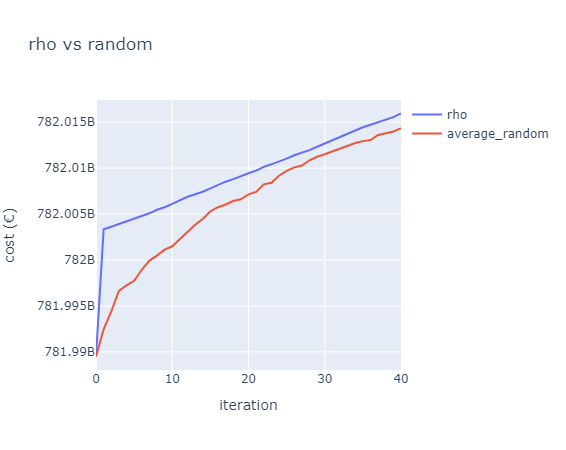
\includegraphics[width=0.8\textwidth]{images/rho_vas_average2.png}
  \caption{Cost variation at each iteration using the \(\rho\) selection method compared to random interval selection.}
  \label{fig:rho_vs_average}
\end{figure}
In plot \ref{fig:val_vs_average}, we compare the cost variation at each iteration using the validation function for interval refinement against the random interval selection method. 
The results indicate that the former method yields a significantly faster increase, implying quicker convergence to the optimal solution. However, this approach incurs greater computational time: \textcolor{red}{many seconds s}. It is worth noting that while both the \(\rho\) and random iteration methods continue even upon encountering a feasible solution for the original problem, the validation function iteration may halt before reaching the maximum iteration limit if the current solution is feasible, thereby being optimal for the original problem.
\begin{figure}[htbp]
  \centering
  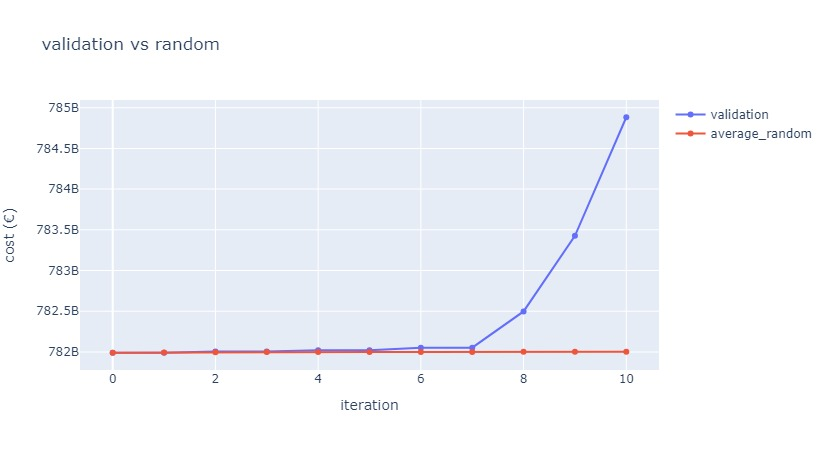
\includegraphics[width=\textwidth]{images/val_vs_average2.png}
  \caption{Cost variation at each iteration using the validation function for interval refinement against the random interval selection method.}
  \label{fig:val_vs_average}
\end{figure}


----- plot same but over real time ----- or just table with time stamps\\
comment: the model takes a lot to set up, but iterations are quick: we are indeed using warm start successfully.



-----plot at each iteration the optimization time trend-------
}




%=================================================================================================================================================================================================================================================================================================================
%=================================================================================================================================================================================================================================================================================================================


%=================================================================================================================================================================================================================================================================================================================
%=================================================================================================================================================================================================================================================================================================================









\section{Conclusion and Future Directions}

{\color{violet}


}













%\begin{acknowledgements}
%If you'd like to thank anyone, place your comments here
%and remove the percent signs.
%\end{acknowledgements}


% Authors must disclose all relationships or interests that 
% could have direct or potential influence or impart bias on 
% the work: 
%
% \section*{Conflict of interest}
%
% The authors declare that they have no conflict of interest.


% BibTeX users please use one of
%\bibliographystyle{spbasic}      % basic style, author-year citations
\bibliographystyle{spmpsci} % mathematics and physical sciences
%\bibliographystyle{spphys}       % APS-like style for physics
\bibliography{sample}   % name your BibTeX data base

% Non-BibTeX users please use
% \begin{thebibliography}{}
% %
% % and use \bibitem to create references. Consult the Instructions
% % for authors for reference list style.
% %
% \bibitem{RefJ}
% % Format for Journal Reference
% Author, Article title, Journal, Volume, page numbers (year)
% % Format for books
% \bibitem{RefB}
% Author, Book title, page numbers. Publisher, place (year)
% % etc
% \end{thebibliography}






%=================================================================================================================================================================================================================================================================================================================
%=================================================================================================================================================================================================================================================================================================================

%                                               APPENDIX

%=================================================================================================================================================================================================================================================================================================================
%=================================================================================================================================================================================================================================================================================================================















\newpage
\color{black}

\appendix

\section{SCENARIO GENERATION}\label{generation}

To estimate the optimal capacities for the CEP through a stochastic approach, realistic and diverse weather scenarios are needed, so to capture the variability and uncertainty of power generation through renewable sources over extended periods. 
In order to generate such scenarios, samples are extracted from a joint probability density function (PDF) fit on historical data. 
%In the following, we use \(Y_t\) to denote the stochastic process of generated power observations for either solar or wind in a single country.
In our project, we used an hourly time step ($T=8760$) and fit the wind and solar distributions separately for each country considered.

To model the marginal probability distributions corresponding to the power output of wind turbines for each hour of the year, a Weibull distribution was used, justified by its proven effectiveness in capturing the variability and skewness of wind power distributions \textcolor{green}{\cite{weibullwind}}. 
For solar power, Beta distributions were employed, as in \textcolor{green}{\cite{betaPV}}.
To fit our model, we used a dataset containing 30 years of data for various European countries, which was collected by \textcolor{green}{\cite{30y_gen}}. 
On the other hand, electricity load is taken from the \textcolor{green}{\href{https://www.entsoe.eu/data/power-stats/}{ENTSO-E Statistical Reports}}. \textcolor{red}{explain how is HL obtained}
In this simple model, while fitting on historical data we did not account for possible changes in future climate, since the focus lies mostly in the computational aspect.

To account for interdependence between temporally near time steps, we coupled these distributions using a Gaussian Copula approach, which captures the dependencies between hourly power outputs effectively. 
This approach accurately represents the coupled behavior in renewable stochastic systems \textcolor{green}{\cite{GaussCopula}}. 

A possible improvement of the generation process could be to fit wind and PV data jointly in the copula step, potentially also including load scenarios with the generation scenarios through the same approach. 
This would consider dependence between Energy Demand and weather conditions, but it would necessitate of the historical dataset provided for the corresponding grid, and would also further increase computational costs.

%\subsubsection{Stochastic Processes description}
%The stochastic processes of power observations will be denoted as \(Y_t\). Where \(t \in T\), is the set indexing all the random variables which want to be considered jointly.
%We assume that the random variable \(Y_t\) has either a Weibull distribution, in the case of Wind Power, or a Beta distribution in the case of Solar Power. 

\subsection{Parametric Estimation of Wind Power distribution}\label{subsection: weib estim}

The parameters defining the Weibull Distribution are estimated using the Maximum Likelyhood Estimation (MLE). 
The Weibull density function is given by:
\begin{equation}
f(x; \theta, \gamma) = \left(\frac{\gamma}{\theta}\right)x^{\gamma-1}\exp\left(-\left(\frac{x}{\theta}\right)^\gamma\right)
\end{equation}
where \(\theta, \gamma > 0\) are the scale and shape parameters, respectively. 

Given observations \(X_1, \ldots, X_n\), the log-likelihood function is:
\begin{equation}
\log L(\theta, \gamma) = \sum_{i=1}^n \log f(X_i \mid \theta, \gamma)
\end{equation}

The optimum solution is found by searching for the parameters for which the gradient is zero:
\begin{equation}
\frac{\partial \log L}{\partial \theta} = -\frac{n \gamma}{\theta} + \frac{\gamma}{\theta^2} \sum_{i=1}^{n} x_i^\gamma = 0
\end{equation}

Eliminating $\theta$, we get:
\begin{equation}
\left[ \frac{\sum_{i=1}^{n} x_i^\gamma \log x_i}{\sum_{i=1}^{n} x_i^\gamma} - \frac{1}{\gamma} \right] = \frac{1}{n} \sum_{i=1}^{n} \log x_i
\end{equation}

This can be solved to get the MLE estimate $\hat{\gamma}$. 
This can be accomplished with the aid of standard iterative procedures such as the Newton-Raphson method or other numerical procedures. 
This is done with the aid of the package \emph{scipy}.
Once $\hat{\gamma}$ is found, $\hat{\theta}$ can be determined in terms of $\hat{\gamma}$ as:
\begin{equation}
\hat{\theta} = \left( \frac{1}{n} \sum_{i=1}^{n} x_i^{\hat{\gamma}} \right)^{\frac{1}{\hat{\gamma}}}
\end{equation}



%%%%%%%%%%%%%%%%%%%%%%%%%%%%%%%%%%%%%%%%%%%%%%%%%%%%%%%%%%%%%%%%%%%%%%%%%%%



\subsection{Parametric Estimation of Solar Power distribution}\label{subsection: beta estim}

To estimate the \(\alpha\) and \(\beta\) parameters defining the Beta distribution \(Y\), we use the Method of Moments.
The mean of the random variable \(Y\) can be expressed as \(\E\left[ Y\right] = \frac{\alpha}{\alpha + \beta} \) and the variance as \(\var [Y]= \frac{\alpha + \beta}{(\alpha + \beta)(\alpha + \beta + 1)}\). 
In particular by explicating \(\beta\) in the first equation and substituting it in the second equation we obtain that:
\begin{equation}
\begin{cases}
\alpha = \mathbb{E}[X] \left( \frac{\mathbb{E}[X](1 - \mathbb{E}[X])}{\mathrm{Var}[X]} - 1 \right) \\
\beta = (1 - \mathbb{E}[X]) \left( \frac{\mathbb{E}[X](1 - \mathbb{E}[X])}{\mathrm{Var}[X]} - 1 \right)
\end{cases}
\end{equation}
By substituting the mean and the variance with their empirical approximation we obtain the Method of Moments estimator for \(\alpha\) and \(\beta\).



%%%%%%%%%%%%%%%%%%%%%%%%%%%%%%%%%%%%%%%%%%%%%%%%%%%%%%%%%%%%%%%%%%%%%%%%%%%



\subsection{Parametric Copula Estimation}
The cumulative density function of both the Weibull and Beta distributions are continuous and invertible. 
Therefore, the random variables \( U_t \coloneqq F_{Y_t}(Y_t) \) have a uniform distribution over \([0,1]\). 
The copula of the random variables \(\{Y_t\}_{t \in T}\) is defined as the function \(C: [0,1]^T \to [0,1]\) such that 
\begin{equation}
C(F_{Y_1}(y_1), \ldots, F_{Y_T}(y_{|T|})) = P(Y_1 \leq y_1, \ldots, Y_{|T|} \leq y_{|T|}).
\end{equation}
This function always exists because of Sklar's Theorem \textcolor{green}{[?]}. 
For a given correlation matrix \(\Sigma\), the Gaussian Copula with parameter matrix \(\Sigma\) is defined as 
\[\CG(u_1,\ldots,u_{T}) \coloneqq \Phi_{\Sigma}(\Phi^{-1}(u_1),\ldots, \Phi^{-1}(u_T)),\] 
where \(\Phi,\; \Phi_{\Sigma}\) are the cumulative distribution functions of Gaussian variables having distribution \(\mathcal{N}(0,1)\) and \( \mathcal{N}(\mathbf{0},\Sigma)\) respectively. 
In particular if \(\CG\) is the copula associated with the random variables \(\{Y_t\}_{t \in T}\) then we have that the random variables \(Z_t = \Phi^{-1}(F_{Y_t}(Y_t)) = \Phi^{-1}(U_t)\) have joint distribution equal to \(\mathcal{N}(0, \Sigma)\). 
This follows from:
\begin{align*}
P(Z_1 \leq z_1, \ldots, Z_T \leq z_t) &= P(\Phi^{-1}(U_1) \leq z_1, \ldots, \Phi^{-1}(U_T) \leq z_T) = \\
&= P(U_1 \leq \Phi(z_1), \ldots, U_T \leq \Phi(z_T)) = \\
&= \CG(\Phi(z_1), \ldots, \Phi(z_t)) =  \\
&= \Phi_{\Sigma}(z_1, \ldots, z_T)
\end{align*}
In particular, given the realization \(\{y_{t,j}\}_{t \in t, j \in J}\) of the variables \(\{Y_t\}_{t \in T}\), an unbiased estimation of the parameter matrix \(\Sigma\) is the empirical covariance matrix \(\hat \Sigma\) of the samples \(\{\Phi^{-1}(\hat{F}_{Y_t}(y_{t,j}))\}_{t\in T, j \in J}\), where \(\hat{F}_{Y_t}\) is the estimated marginal distribution of the variable \(Y_t\) obtained as seen in sections \ref{subsection: weib estim} and \ref{subsection: beta estim}.

Finally, we can generate samples from a Multivariate Gaussian random variable \((Z_{t}, t \in T)\) having distribution \(\mathcal{N}(0, \hat \Sigma)\).
Then the power output scenarios are obtained from these samples by following the previous steps backwards, that is, for each sample, computing \(\hat F_{t}^{-1}(\Phi(Z_{t}))\) for all \(t\in T\). 













%=================================================================================================================================================================================================================================================================================================================
%=================================================================================================================================================================================================================================================================================================================


%=================================================================================================================================================================================================================================================================================================================
%=================================================================================================================================================================================================================================================================================================================
















\section{STRUCTURE PRESERVING CONTRAINT TRASFORMATIONS}\label{appendix B}

Questa parte è la teoria sviluppata da Gabor. Non la metto nella mia tesi, la riserviamo per l'articolo.











\end{document}
% end of file template.tex

